\documentclass[11pt]{article}

\usepackage[activate={true,nocompatibility},final,tracking=true,kerning=true,spacing=true,factor=1100,stretch=10,shrink=10]{microtype}
\usepackage{multirow}
\usepackage{mathtools}
\usepackage{graphicx}
\usepackage{tabularx}
\usepackage{enumerate}
\usepackage{amsmath, amssymb, graphics, setspace}
\usepackage[noline,noend,ruled,linesnumbered]{algorithm2e}
\usepackage{algpseudocode}
\usepackage{enumitem}

\DeclareMathOperator{\lcm}{lcm}

\newcommand{\mathsym}[1]{{}}
\newcommand{\unicode}[1]{{}}

\title{Assignment 3}

\author{Paul Jones and Matthew Klein \\
		Professor Kostas Bekris\\
		Design and Analysis of Computer Algorithms (01.198.344)}

\date{\today}

\usepackage{setspace}
\singlespacing

\usepackage[letterpaper]{geometry}
\geometry{top=1in, bottom=1in, left=.5in, right=.5in}

\usepackage{fancyhdr}
\pagestyle{fancy}
\lhead{Paul Jones and Matthew Klein \\ Professor Kostas Bekris}
\chead{}
\rhead{Design and Analysis of Computer Algorithms \\ Rutgers University}
\lfoot{}
\cfoot{\thepage}
\rfoot{}

\begin{document}

\pagebreak

\section*{Part A (35 points)}

\subsection*{Problem 1} You are participating in the design of a
new stepping stones challenge for the remake of the cult Japanese TV
show ``Takeshi's Castle''.\\

\noindent The challenge involves a team of two people tied with a rope
that need to walk over a sequence of stepping stones. The first
teammate is allowed to go over the stepping stones that are painted
red $\{r_0, \ldots, r_n\}$, while the second teammate is allowed to go
over the stepping stones that are painted blue $\{b_0, \ldots,
b_m\}$. For the team to win, the two players have to walk over all the
stepping stones in the corresponding sequence while they are connected
with the rope. The teammates are not allowed to backtrack. At each
point in time, either one of the players can jump from her current
stone to the next one and the other one stays at his current stone, or
both of them jump simultaneously from their current stones to the next
ones. Such a jump is obviously feasible only if the distances between
the two players before and after the jump are less than the length of
the rope connecting them.\\

\noindent The TV show producer has already built the two sequences of
red and blue stepping stones. Given the coordinates of the stepping
stones, your task is to select the minimum length of the rope for
which it is possible for the two players to win the game. This is what
will make the show entertaining for the audience!\\

\noindent \textbf{Provide an algorithm for this computation and argue its
running time.}


This problem is the same as the edit distance but instead of two words we have from $r_0,r_n$ and $b_0,b_n$. Similar to that problem from class, we must solve a prefix of $r_0,r_j$ and $b_0,b_j$. There are three sub problems: $r[j]$ and a gap, $b[j]$ and a gap, or $r[j],b[j]$ meaning they are the same or different and nothing needs to be added. We can use what is in the DPV book, $E(i,j) = min\{1+E(i-1,j), 1+E(i,j-1), diff(i,j)+E(i-1,j-1)\}$. where $diff$ is the difference, $0$ if they are the same and $1$ if they are different. Rather than finding the edit distance for words, we find the edit difference between the movements. Our max number, $n$, is the length of the rope. If we need to add a gap, we increase by one. If they jump together, then we do not. The largest this distance can be is the length of the rope. Because of this, the total running time to compute this is $O(nm)$.

\section*{Part B (35 points)}

\subsection*{Problem 2}

\begin{enumerate}[label=\Alph*.]

\item \textbf{You have a collection of $n$ distinct chopsticks of
length $l_{1},\dots,l_{n}$. Any two of them can be paired for use if
the length of them differ at most $k$. How can you easily pair as many
of the chopsticks as possible? Describe a greedy algorithm of time
complexity $O(n\log n)$ to solve this problem and prove the
correctness of your algorithm.}\\

\item \textbf{Consider now a variant of the above problem. You
can still only pair chopsticks that differ at most $k$ in length. But
now a value $w_{i}$ is also associated with each individual
chopstick. You want to maximize the sum of the values of the
chopsticks that have been paired.}\\

\noindent For example, suppose you have 7 chopsticks of length
$5,2,3,11,9,12,16$ and corresponding values $1,1,2,5,3,3,10$. You are
allowed to pair chopsticks that differ by at most 3 units in
length. Then one of the optimal solutions here is $\{ (2,3),(9,11) \}$
of optimal value $1+2+3+5=11$.\\

\noindent How can you pair the chopsticks so as to maximize the value?
Describe a dynamic programming algorithm of time complexity $O(n^{2})$
to solve this problem. Can you do better than $O(n^{2})$?\\

\noindent \textbf{Describe a greedy algorithm of time
complexity $O(n\log n)$ to solve this problem and prove the
correctness of your algorithm.}\\

A greedy algorithm for this would be to take every chopstick $n_i$ and a second one, $n_j$ that differ by $k$ as many times as possible. When we run out of two pairs $i,j$ that are different by $k$, we take two pairs that differ by $k-i$ until the set is empty. This is our greedy algorithm. This takes $O(n\log n)$. Why? Because each time we're taking 2 chopsticks (a tree basically) and we continue this $n$ times.

\noindent \textbf{Describe a dynamic programming algorithm of time complexity $O(n^{2})$ to solve this problem. Can you do better than $O(n^{2})$?}\\

A dynamic programming algorithm for this is similar to the knapsack problem. $K(w,j) = max\{K(w-wk,j-1) + v_j,K(w,j-1)\}$ where $0 \leq j \leq n$. $K$ is the "knapsack" in this problem, or holding the chopsticks. Rather than taking each chopstick, we take two at a time. This is $O(nW)$. \\
\\
It is possible to do better than $O(n^2)$ just by using a sort function on the chopsticks and pairing the best match (from our greedy algorithm).

\end{enumerate}

\section*{Part C (20 points)}

\subsection*{Problem 3} In the robotics lab the new robot has just
arrived. The robot has the ability to construct a topological map of
the environment, such as the graph shown in Figure
\ref{fig:problem3}. The robot is allowed to move only forward along
the directions of the edges on the topological map. Moreover, the
graph is being constructed in such a way that will prevent the robot
to execute loops, i.e., the robot is not able to visit a node that it
has already visited.\\

\begin{figure}[h]
  \centering
  \caption{An example of a directed graph that the robot build for this map.}
    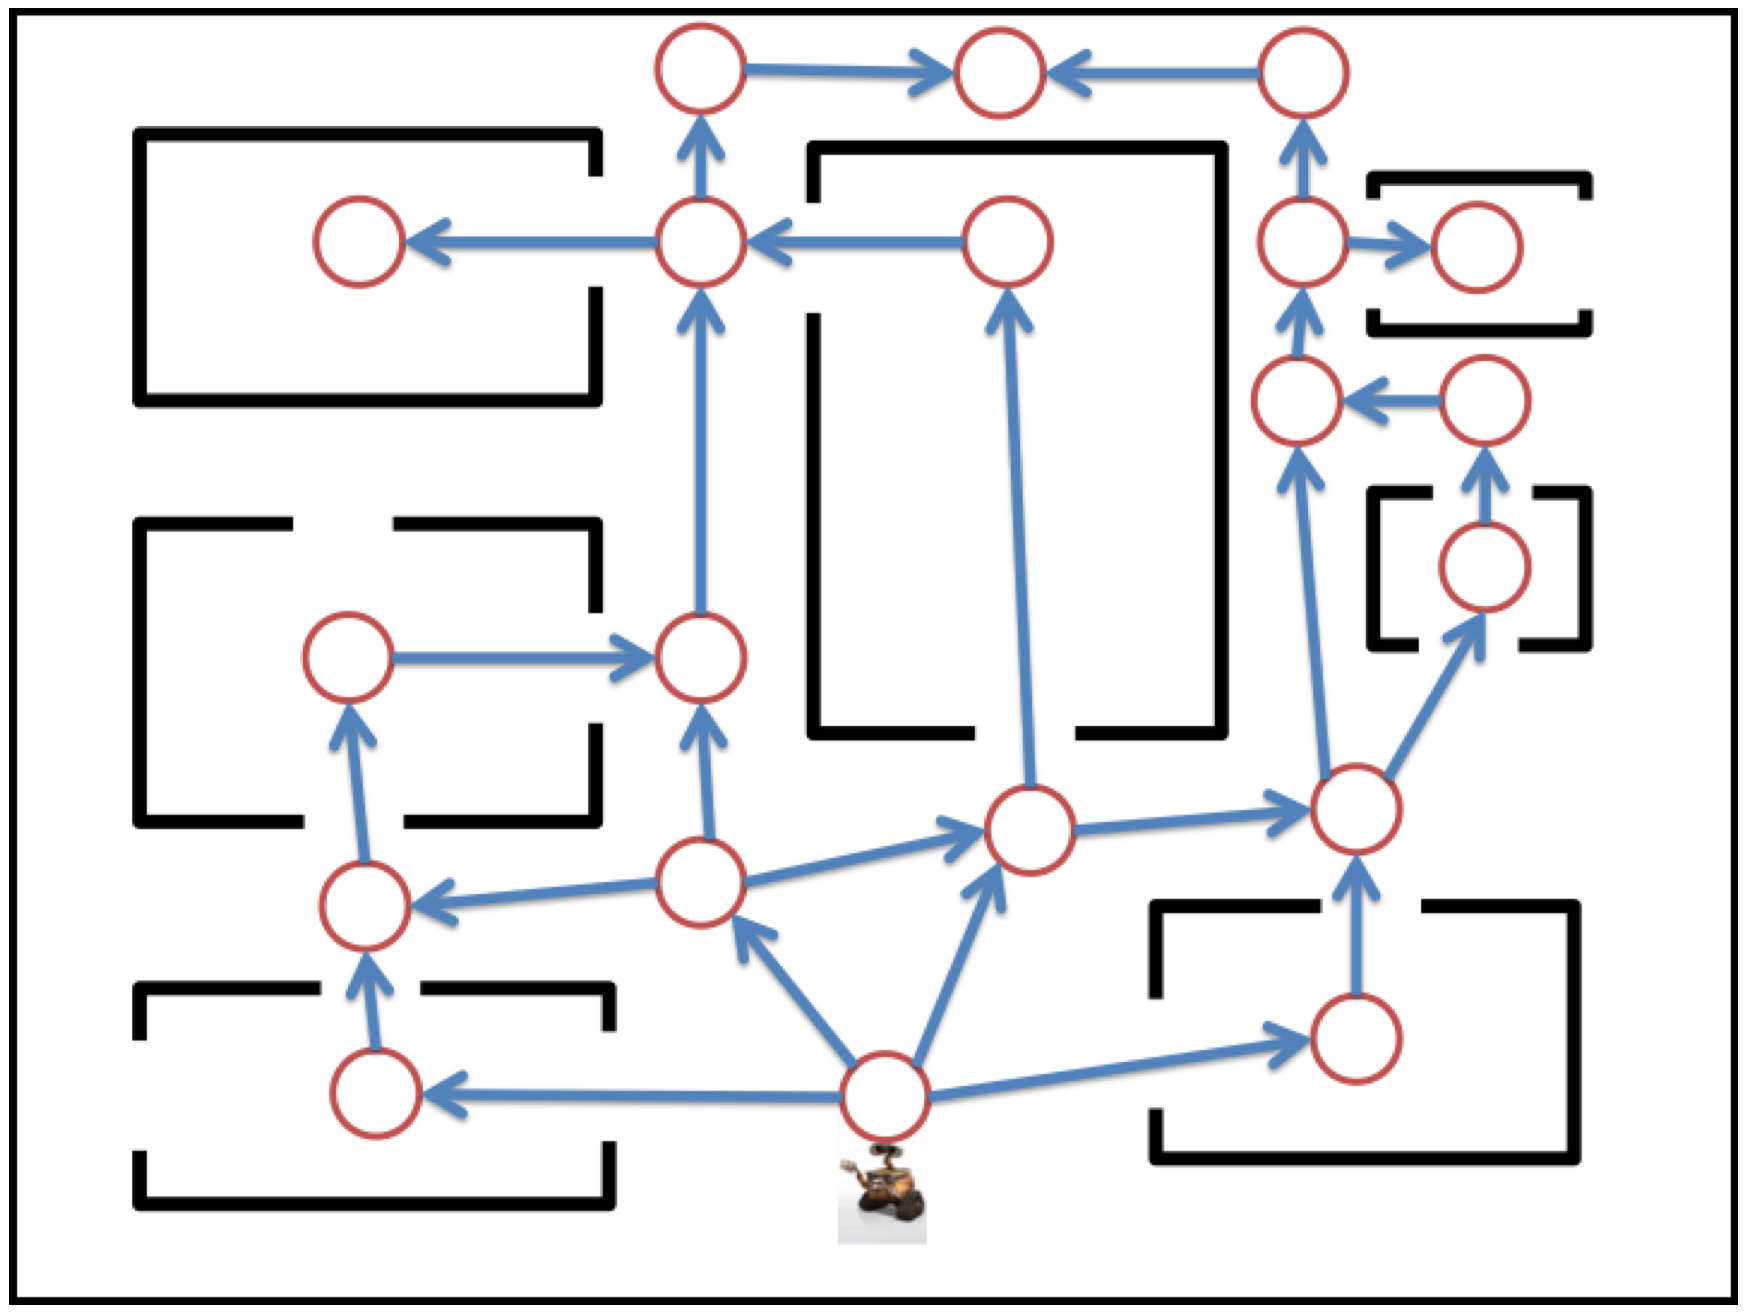
\includegraphics[width=0.5\textwidth]{paths}
    \label{fig:problem3}
\end{figure}

\begin{enumerate}[label=\Alph*.]

\item \textbf{Given a start location for your robot and a target
location, provide an efficient algorithm that will return all the
possible paths from the start to the target.  What is the running time
for your algorithm?}

\begin{verbatim}
def find_all_paths(graph, start, end, path=[]):
    path = path + [start]
    if start == end:
        return [path]
    paths = []
    for node in graph[start]:
        if node not in path:
            newpaths = find_all_paths(graph, node, end, path)
            for newpath in newpaths:
                paths.append(newpath)
    return paths 
\end{verbatim}

\item \textbf{You want to check if the topological map provides
enough information for your robot to be able to visit all the rooms so
as to clean them. Provide an efficient algorithm that will be able to
check if there is a path for the robot on the graph that can visit all
the rooms (i.e., nodes on the graph).}
\end{enumerate}

Wikipedia:
\begin{enumerate}
\item Begin at any arbitrary node of the graph, G
\item Proceed from that node using either depth-first or breadth-first search, counting all nodes reached.
\item Once the graph has been entirely traversed, if the number of nodes counted is equal to the number of nodes of G, the graph is connected; otherwise it is disconnected.
\end{enumerate}
\section*{Part D (20 points)}

\subsection*{Problem 4} You are preparing a banquet where the
guests are government officials from many different countries. In
order to avoid unnecessary troubles, you are asked to check the list
of international conflicts in the last ten years. Then, you will
assign the guests to two tables, such that in each table, any two
guests are not from countries that had conflicts in the last ten
years.\\

\noindent \textbf{Provide an efficient algorithm that determines whether it is
possible to make such an assignment. If it is possible to do so, the
algorithm should return the assignment of these two tables. What is
the running time?}

\end{document}

